\documentclass[main.tex]{subfiles}
\begin{document}

\begin{frame}{Statistika Perencanaan}
	\begin{columns}[c]
		\begin{column}{.5\textwidth}
			\begin{figure}
				\centering
				\includegraphics[width=0.8\textwidth]{figures/statistik}
				% \caption{Block diagram of a 1st order system.}
			\end{figure}
		\end{column}
		\begin{column}{.5\textwidth}
			\begin{figure}
				\centering
				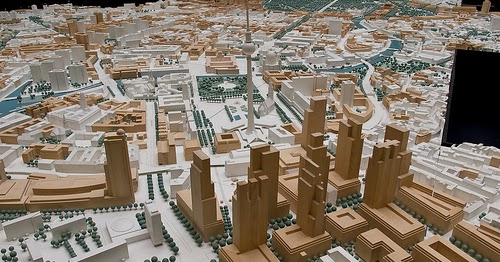
\includegraphics[width=0.8\textwidth]{figures/planologi}
				% \caption{Step response of a 1st order system.}
			\end{figure}
		\end{column}
	\end{columns}
\end{frame}

\begin{frame}[c]
	\large Statistik berkaitan dengan
	\begin{enumerate}
		\item \textcolor{red}{Angka – angka}
		\item Data
		\item \textcolor{blue}{Informasi}
	\end{enumerate}
	\large Perbedaan
	\textbf{data} dan \textbf{informasi}
\end{frame}

\begin{frame}[c]
	\begin{figure}
		\begin{center}
			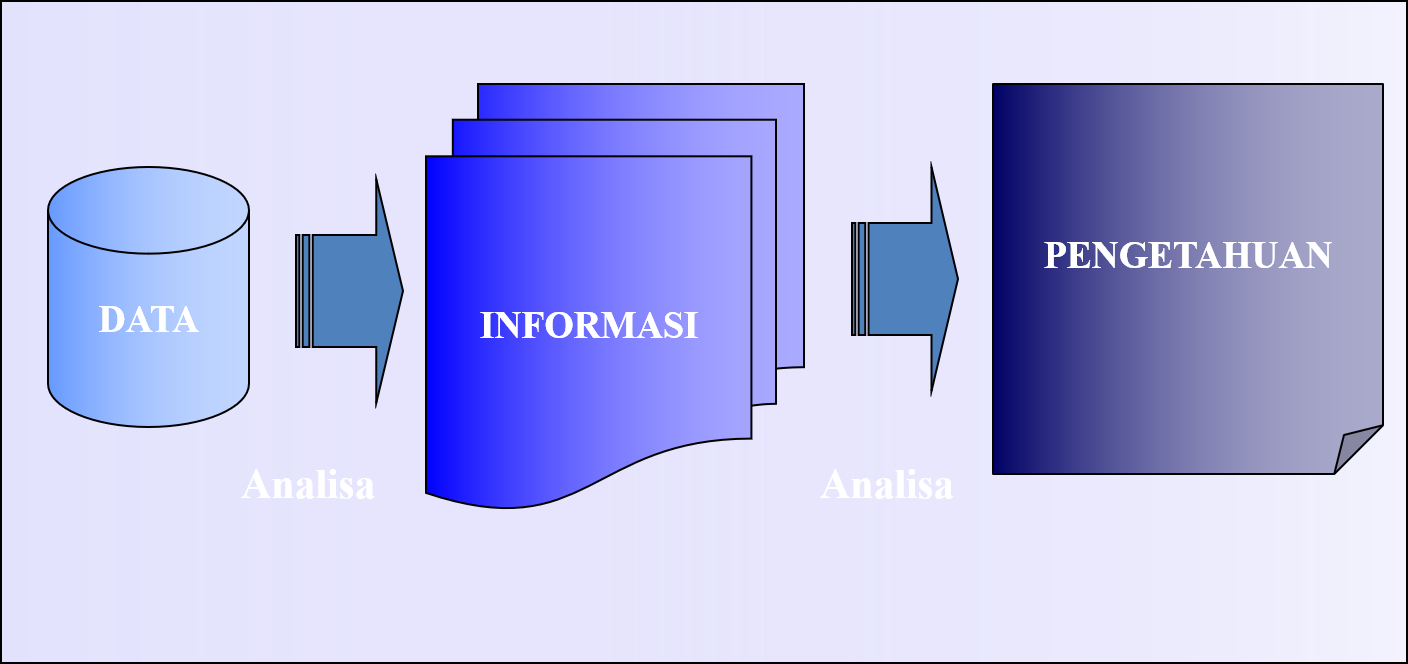
\includegraphics[height=2in]{figures/data}
		\end{center}
	\end{figure}
\end{frame}

\begin{frame}[t]
	\frametitle{data}
	\framesubtitle{pengertian Data}
	\begin{textblock*}{2cm}(10cm,7cm) % {block width} (coords.12,8cm)
		
\includegraphics[width=2cm]{figures/cons}
	\end{textblock*}
	% Pengertian data
	Data adalah sesuatu yang \textit{diketahui} atau \textit{dianggap}, dengan demikian data dapat memberikan gambaran tentang suatu keadaan atau persoalan.
	\begin{enumerate}
		\item Dasar membuat keputusan \textit{(decision makers)}
		\item Dasar perencanaan
		\item Alat pengendalian
		\item Dasar evaluasi
	\end{enumerate}
	\notec{Misalnya; data mahasiswa : sesuatu yang dapat memberikan informasi tentang mahasiswa: jenis kelamin, usia, IPK rata-rata, fakultas, jurusan dsb. }
\end{frame}

\begin{frame}[c]
	\frametitle{data}
	\framesubtitle{manfaat}
	\begin{itemize}
		\item Memberikan informasi tentang suatu keadaan
		\item Sebagai  dasar objektif  dalam proses pemuatan keputusan/kebijakan dalam rangka  pemecahan masalah.

	\end{itemize}
\end{frame}

\begin{frame}[c]
	\frametitle{data}
	\framesubtitle{kriteria}
	\begin{textblock*}{40mm}(.5cm,4cm) % {block width} (coords.12,8cm)
		
\includegraphics[width=20pt]{figures/ver}
	\end{textblock*}
	\begin{textblock*}{30pt}(.5cm,6cm) % {block width} (coords.12,8cm)
		
\includegraphics[width=20pt]{figures/rel}
	\end{textblock*}

	\begin{description}
		\item[Valid]: menunjukkan derajat ketepatan antara data yang sesungguhnya terjadi pada objek dengan data yang dikumpulkan peneliti.
		\item[Reliabel]: berkenaan dengan derajat konsistensi/keajegan data dalam interval waktu tertentu
	\end{description}

\end{frame}

\begin{frame}[t]
	\frametitle{data}
	\framesubtitle{kriteria data yang baik}
	\begin{description}
		\item [Objektif], berarti data harus sesuai dengan keadaan yang sebenarnya (as it is).
		\item [Representatif] (mewakili), data harus mewakili objek yang diamati.
		\item [Kesalahan baku (standard error) yang kecil], suatu perkiraan (estimate) dikatakan baik apabila kesalahan bakunya kecil.
		\item [Tepat waktu], agar dapat dilakukan koreksi
		\item [Relevan], data yang dikumpulkan harus ada hubungannya dengan masalah yang akan diteliti (dipecahkan)
	\end{description}
\end{frame}

\begin{frame}[c]
	\frametitle{data}
	\framesubtitle{jenis}
	Menurut sifatnya:
	\begin{description}
		\item[Data kualitatif]: yaitu informasi  yang tidak berbentuk angka dinyatakan dalam kalimat  atau keterangan.
		\item [Data kuantitatif]: informasi yang disusun dalam bentuk angka.
	\end{description}
	\textit{Contoh : sepertiga  penduduk Jakarta adalah  nelayan}

\end{frame}

\begin{frame}[c]
	\frametitle{data}
	\framesubtitle{jenis}
	\begin{description}
		\item[Diskrit] : data  yang selalu memiliki nilai bulat dalam bilangan asli, tidak pecahan. Atau data yang tidak mengambil seluruh nilai dalam sebuah interval (selang)
		\item[Kontinum] : data yang memiliki nilai sembarang baik bulat maupun pecahan. data yang mengambil seluruh nilai dari selang.
	\end{description}
	\textit{tinggi badannya 167,40 cm,  berat badan 50,5 kg}
	\begin{textblock*}{2cm}(10cm,7cm) % {block width} (coords.12,8cm)
		
\includegraphics[width=2cm]{figures/cons}
	\end{textblock*}
\end{frame}

\begin{frame}[c]
	\frametitle{data}
	\framesubtitle{bagan}

	\begin{figure}
		\begin{center}
			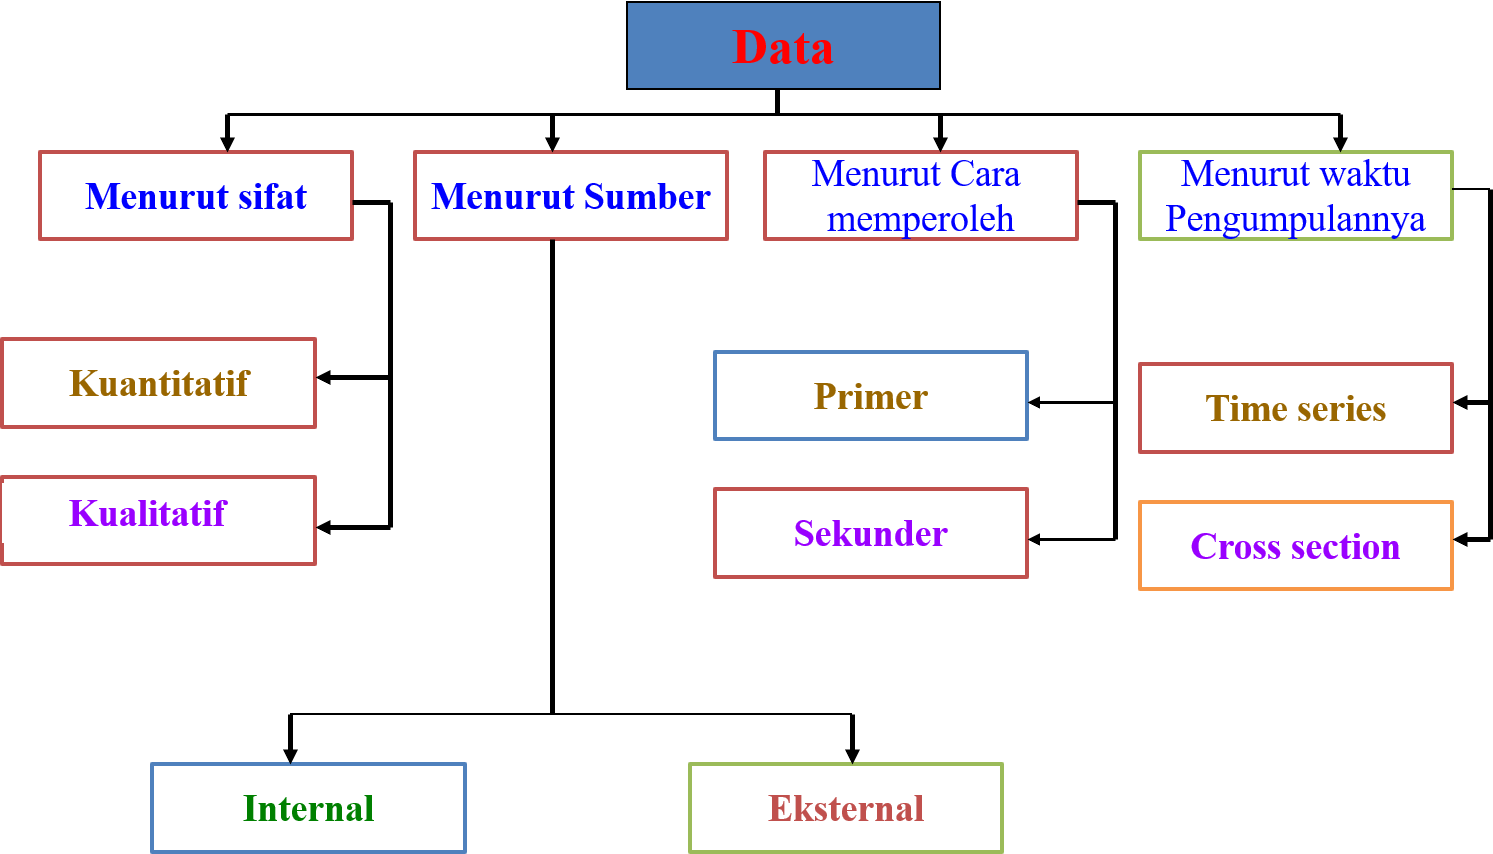
\includegraphics[scale=.4]{figures/bagan}
		\end{center}
	\end{figure}
\end{frame}
\begin{frame}[c]
	\frametitle{data}
	\framesubtitle{jenis}
	Menurut cara memperolehnya:
	\begin{description}
		\item[Data primer] yaitu informasi  yang dikumpulkan dari tangan pertama (firsthand).
			Contoh:  data yang berasal dari hasil jawaban kuesionoer, misalnya data tanggapan kepuasan konsumen, dan data yang dicatat dari hasil pengamatan peneliti.
		\item[Data sekunder] yaitu informasi yang diperoleh dari publikasi yang telah dilakukan oleh pihak lain
			Contoh:  Data nilai penjualan yang diambil dari laporan keuangan, inflasi, volume penjualan, dsb.
	\end{description}
\end{frame}

\begin{frame}[c]
	\frametitle{jenis data menurut cara memperolehnya}
	\framesubtitle{data primer}

	\begin{textblock*}{2cm}(10cm,7cm) % {block width} (coords.12,8cm)
		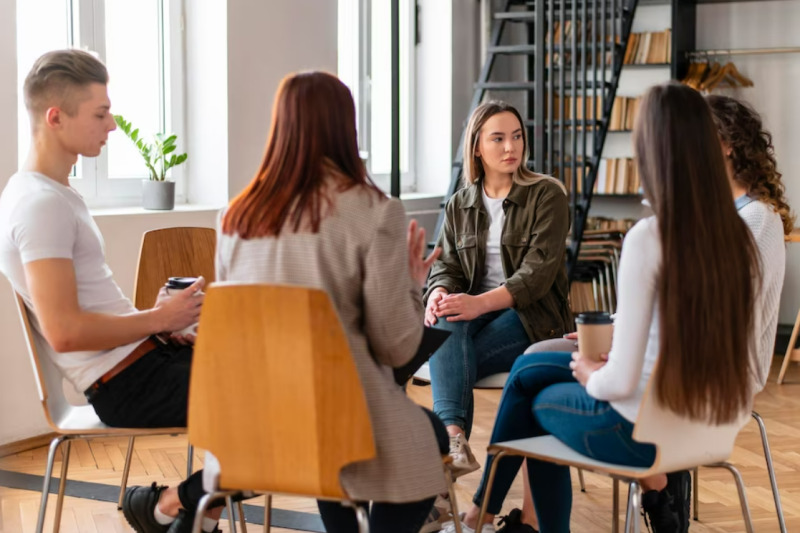
\includegraphics[width=2cm]{figures/fgd}
	\end{textblock*}
	\begin{columns}
		\begin{column}{0.5\textwidth}
			\begin{itemize}
				\item Data Primer merupakan sumber data penelitian yang diperoleh secara langsung dari sumber asli (tidak melalui media perantara.
				\item Data primer secara khusus dikumpulkan oleh peneliti untuk menjawab pertanyaan penelitian.
			\end{itemize}
		\end{column}

		\begin{column}{0.5\textwidth}
			Teknik yang pada umumnya dipergunakan adalah dengan :
			\begin{itemize}
				\item Observasi
				\item Wawancara
				\item Kuesioner
				\item Dokumenter
			\end{itemize}
		\end{column}
	\end{columns}
	\notec{\tabitem Metode yang bisa dipergunakan untuk mengumpulkan data primer adalah dengan studi lapangan.}
\end{frame}

\begin{frame}[c]
	\frametitle{jenis data}
	\framesubtitle{data sekunder}
	\begin{columns}
		\begin{column}{0.5\textwidth}
			\begin{itemize}
				\item Data sekunder merupakan sumber data penelitian yang diperoleh peneliti secara tidak langsung melaui media perantara (diperoleh dan dicatat oleh pihak lain)
			\end{itemize}
		\end{column}
		\begin{column}{0.5\textwidth}
			\begin{itemize}
				\item Data sekunder umumnya berupa bukti, catatan atau laporan historis yang telah disusun dalam arsip (data dokumenter) yang dipublikasikan dan yang tidak dipublikasikan.
			\end{itemize}
		\end{column}
	\end{columns}
	\notec{Metode yang dipergunakan untuk pengumpulan data sekunder ini adalah dengan studi kepustakaan.}
\end{frame}

\begin{frame}[c]
	\frametitle{data}
	\framesubtitle{jenis}
	Menurut waktunya
	\begin{description}
		\item[cross section] yaitu kumpulan informasi yang berasal dari satu waktu
		\item[time series] yaitu kumpulan informasi yang berasal dari deretan waktu. Periode waktu dapat berupa harian, mingguan, bulanan, kuartalan, semesterean dan tahunan.
	\end{description}
\end{frame}

\begin{frame}[c]
	\frametitle{definisi statistik}
	\begin{block}{}
		Berasal dari bahasa latin ``status" : negara.
	\end{block}
	\begin{block}{}
		Berkaitan dengan penyajian data atau fakta – fakta tentang perekonomian, kependudukan, dan politik suatu negara.
	\end{block}
\end{frame}

\begin{frame}[c]
	\frametitle{definisi statistik}
	\framesubtitle{Dalam arti sempit,}
	Data ringkasan yang berbentuk angka (kuantitatif), misal statistik penduduk, adalah data atau keterangan berbentuk angka ringkasan mengenai penduduk (jumlah, rata-rata masa kerja, rata-rata jumlah anggota keluarga, persentase yang sarjana) dan sebagainya.
\end{frame}

\begin{frame}[c]
	\frametitle{definisi statistik}
	\framesubtitle{Dalam arti luas,}
	Ilmu yang mempelajari cara pengumpulan, pengolahan /pengelompokan, penyajian dan analisis data serta cara pengambilan simpulan secara umum berdasarkan hasil penelitian yang tidak menyeluruh.
\end{frame}

\begin{frame}[c]
	\frametitle{Penggunaan Statistika}
	Statistika banyak diterapkan dalam berbagai disiplin ilmu:

	\begin{itemize}
		\item Ilmu – ilmu alam
		\item Ilmu – ilmu sosial
		\item Ekonomi
		\item Pemerintahan
		\item Komputasi, dll
	\end{itemize}
\end{frame}

\begin{frame}[c]
	\frametitle{Peran Komputer dalam Statistik}
	\framesubtitle{Software}
	\begin{itemize}
		\item Jumlah masukan (input) yang besar
		\item Proyek yang repetitif
		\item Diinginkan dan diperlukan kecepatan yang tinggi dalam pengolahannya
		\item Diinginkan dan diperlukan ketepatan yang lebih besar
		\item Mengolah hal-hal kompleks yang memerlukan bantuan elekrtonik
	\end{itemize}
	\notec{Minitab, SAS, SPSS (sering dipakai mahasiswa khususnya untuk Skripsi) dan SYSTAT}
	\notec{cari tahu software software ini}
\end{frame}

\begin{frame}[c]
	\frametitle{Peran Statistik}
	\begin{itemize}
		\item Menyediakan informasi dalam bentuk      yang luas dan formal
		\item Mengukur banyak hal dalam berbagai bidang dalam bentuk angka/numerik (indikator)
		\item Mengukur banyak variasi dalam proses biologi
	\end{itemize}
\end{frame}

\begin{frame}[c]
	\frametitle{Ruang Lingkup Statistik}
	\begin{enumerate}[(a)]
		\color{blue}
		\item Statistik Deskriptif
		\item Statistik Inferensial
	\end{enumerate}
	\notec{cth deskriptif}
	\notec{\tabitem Menghitung rata – rata dan varians dari data mentah}
	\notec{\tabitem Mendeksripsikan menggunakan tabel – tabel atau grafik sehingga data mentah lebih mudah “dibaca” dan lebih bermakna.  }
	\notec{cth inferensial}
	\notec{\tabitem Pengujian hipotesis
		\tabitem Melakukan estimasi pengamatan masa mendatang (estimasi atau prediksi)
		\tabitem Membuat permodelan hubungan           (korelasi, regresi, ANOVA, deret waktu),      dsb }
\end{frame}









%   \tiny Weiteres dazu entnehmen Sie bitte dem Infoblatt: \url{http://www.virtuelle-ph.at/selbst-electures-abhalten/infoblatt}

%   \small Die Teilnehmenden werden über einen Disclaimer zu Beginn der eLecture darüber informiert:

\end{document}
